% Компіляція: lualatex -shell-escape main.tex (двічі)
\documentclass[12pt,a4paper]{article}

\usepackage{fontspec}
\usepackage{polyglossia}
\setdefaultlanguage{ukrainian}
\setmainfont{NewComputerModern10}
\setsansfont{Noto Sans}
\setmonofont{Noto Sans Mono}[Scale=0.82]

\usepackage{amsmath,amssymb,array,booktabs,caption,enumitem,float,geometry,graphicx,microtype,titlesec,xcolor}
\geometry{left=2cm,right=2cm,top=2cm,bottom=2cm}
\setlength{\parindent}{1.25cm}
\linespread{1.08}
\titleformat{\section}{\normalfont\fontsize{14}{16}\selectfont\bfseries}{\thesection}{0.6em}{}
\titleformat{\subsection}{\normalfont\fontsize{12}{14}\selectfont\bfseries}{\thesubsection}{0.6em}{}
\titlespacing*{\section}{0pt}{1.4em}{0.65em}
\titlespacing*{\subsection}{0pt}{1.1em}{0.45em}
\captionsetup{font=small,labelfont=bf,labelsep=endash}
\captionsetup[table]{position=bottom,skip=5pt}

\usepackage[newfloat]{minted}
\SetupFloatingEnvironment{listing}{name=Лістинг}
\setminted{fontsize=\scriptsize,linenos,breaklines,breakanywhere,autogobble,frame=single,framesep=2mm,bgcolor=gray!5,tabsize=4}

\usepackage[unicode,colorlinks=true,linkcolor=black,urlcolor=blue,
  pdftitle={ІО-41, Давидчук Артем, Вступ до штучного інтелекту, Лабораторна робота №4},
  pdfauthor={Давидчук Артем},pdfsubject={Нейронні мережі}]{hyperref}

\begin{document}
\pagenumbering{gobble}
\begin{titlepage}
  \begin{center}
    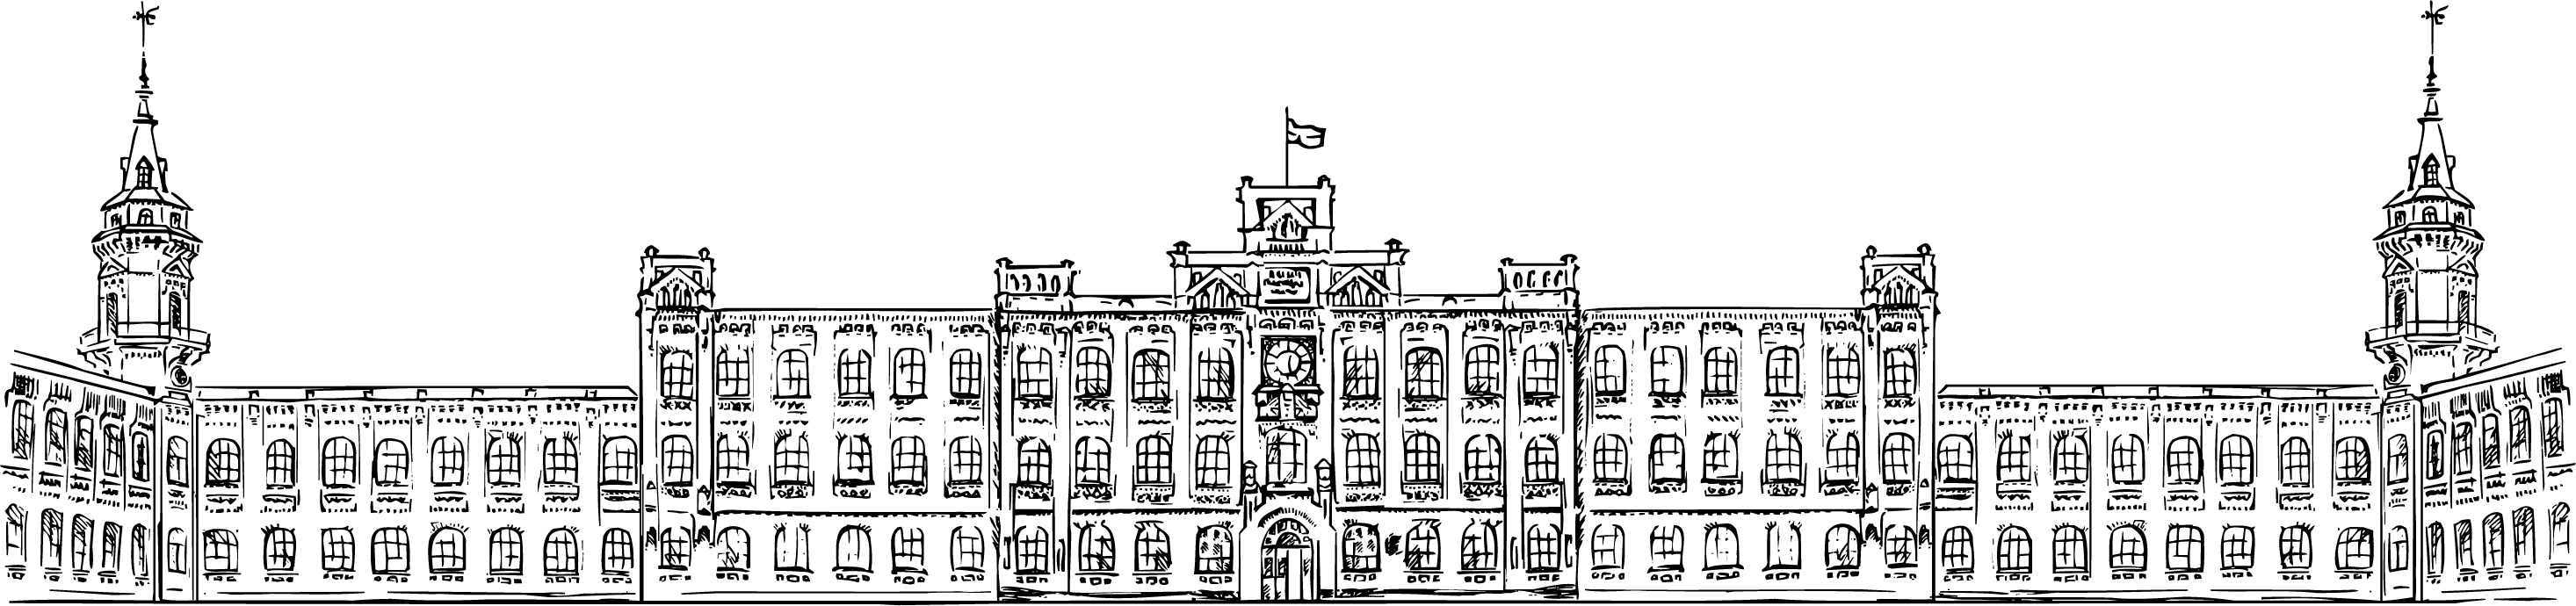
\includegraphics[width=0.7\textwidth]{../../../../../../templates/letterhead.png}
  \end{center}
  \begin{center}
    \large
    Національний технічний університет України\\
    «Київський політехнічний інститут імені Ігоря Сікорського»\\[1em]
    Факультет інформатики та обчислювальної техніки\\
    Кафедра обчислювальної техніки
  \end{center}
  \vfill
  \begin{center}
    \textbf{\LARGE Вступ до штучного інтелекту}\\[2em]
    \textbf{\Large Лабораторна робота №4}\\[0.7em]
    \parbox{0.9\textwidth}{\centering «Нейронні мережі»}
  \end{center}
  \vfill
  \begin{flushright}
    \begin{minipage}{0.48\textwidth}
      Виконав: студент групи ІО-41\\
      \textit{Давидчук Артем}\\[1em]
      Перевірив: \textit{Кочура Ю. П.}
    \end{minipage}
  \end{flushright}
  \vfill
  \begin{center}Київ --- 2026\end{center}
\end{titlepage}
\pagenumbering{arabic}

\section{Мета роботи}

Удосконалити інтелектуального агента --- мережевий контролер із попередньої
лабораторної роботи --- системою визначення пропускної здатності каналів на
основі згорткової нейронної мережі. Набути практичних навичок класифікації
зображень, експорту, квантування й оцінювання швидкодії моделі на CPU.

\section{Постановка задачі}

Кожному ребру графа мережі випадково призначається маркування у вигляді
зображення цифри MNIST від 2 до 9. Цифра $d$ відповідає пропускній здатності
$100d$ Мбіт/с. Контролер перед використанням каналу розпізнає його маркування
згортковою нейронною мережею та враховує отримане значення під час вибору
маршруту для потоку обсягом 1 ГБ.

Необхідно натренувати CNN, експортувати її у формат ONNX, виконати квантування
INT8, перевірити точність і виміряти швидкодію. Сам контролер повинен
використовувати саме квантовану ONNX-модель через CPU Execution Provider.

\section{Теоретичні відомості}

\subsection{Згорткова нейронна мережа}

Згорткова нейронна мережа (CNN) виявляє локальні просторові ознаки зображення.
Згорткові шари формують карти ознак, функція ReLU додає нелінійність, а
MaxPooling зменшує просторовий розмір даних. Після цього повнозв'язні шари
перетворюють ознаки у десять оцінок класів. Прогнозом є індекс найбільшої
оцінки.

Використана модель містить два блоки Conv2D--ReLU--MaxPool, а потім шари
Flatten, Linear(1568, 64), ReLU та Linear(64, 10). Навчання виконується на CPU
оптимізатором Adam і функцією втрат cross-entropy.

\subsection{Експорт та квантування}

ONNX є переносимим форматом представлення обчислювального графа нейронної
мережі. Експортована модель запускається незалежно від тренувального
середовища через ONNX Runtime.

Післятренувальне статичне квантування переводить ваги та активації з FP32 у
8-бітне цілочисельне представлення. Для визначення діапазонів активацій
використано 1000 калібрувальних зображень. Це зменшує розмір моделі й витрати
пам'яті, проте округлення може трохи знизити точність. Виграш у швидкості
залежить від процесора, реалізації операторів і розміру пакета.

\subsection{Розрахунок часу передавання}

Оскільки передавання каналами відбувається конвеєрно, пропускну здатність
усього шляху обмежує найповільніший канал. Для шляху $P$ час передавання
обчислюється за формулою

\begin{equation}
  T(P)=\frac{\sum\limits_{e\in P}d_e}{1000}
       +\frac{8000S}{\min\limits_{e\in P}B_e},
\end{equation}

де $d_e$ --- затримка ребра в мілісекундах, $B_e$ --- розпізнана пропускна
здатність у Мбіт/с, $S$ --- розмір потоку в ГБ. Для цієї роботи $S=1$.

\section{Алгоритм роботи}

Робота програми складається з таких етапів:

\begin{enumerate}[leftmargin=2cm]
  \item завантажити MNIST, зафіксувати генератори випадкових чисел і
        натренувати CNN на CPU;
  \item перевірити точність PyTorch-моделі, експортувати її в ONNX та
        виконати статичне INT8-квантування;
  \item після прогрівання виміряти середній час одного розпізнавання та
        продуктивність пакета з 1000 зображень;
  \item створити граф із ЛР1, випадково призначити ребрам затримки та
        MNIST-маркування цифрами 2--9;
  \item під час TELL додавати відомі канали в базу знань; квантована модель
        розпізнає їхні маркування і зберігає знайдену пропускну здатність;
  \item під час ASK обрати шлях із мінімальним повним часом передавання;
  \item встановлювати правила до досягнення цілі, а за відсутності шляху
        відкликати останнє правило і продовжити пошук;
  \item вивести характеристики каналів шляху, вузьке місце, час
        розпізнавання та сумарний час передавання.
\end{enumerate}

Для пошуку найкращого шляху перебираються можливі пороги пропускної
здатності 200--900 Мбіт/с. Для кожного порога створюється підграф лише з
каналами, пропускна здатність яких не нижча за поріг. У ньому алгоритмом
Дейкстри знаходиться шлях із найменшою сумою затримок, після чого оцінюється
повний час за наведеною формулою. Обирається кандидат із найменшим часом.

\section{Програмна реалізація}

\subsection{Архітектура CNN}

\begin{listing}[H]
\begin{minted}{python}
class MnistCNN(nn.Module):
    def __init__(self):
        super().__init__()
        self.features = nn.Sequential(
            nn.Conv2d(1, 16, kernel_size=3, padding=1), nn.ReLU(),
            nn.MaxPool2d(2),
            nn.Conv2d(16, 32, kernel_size=3, padding=1), nn.ReLU(),
            nn.MaxPool2d(2),
        )
        self.classifier = nn.Sequential(
            nn.Flatten(), nn.Linear(32 * 7 * 7, 64),
            nn.ReLU(), nn.Linear(64, 10),
        )

    def forward(self, images):
        return self.classifier(self.features(images))
\end{minted}
\caption{Архітектура згорткової нейронної мережі}
\end{listing}

\subsection{Експорт і квантування}

Експорт виконується з динамічною віссю розміру пакета, тому одна модель
підтримує як одиночні зображення, так і пакет із 1000 зображень.

\begin{listing}[H]
\begin{minted}{python}
torch.onnx.export(
    model,
    torch.zeros(1, 1, 28, 28, dtype=torch.float32),
    output_path,
    input_names=["images"], output_names=["logits"],
    dynamic_shapes={"images": {0: torch.export.Dim("batch")}},
    opset_version=18,
    dynamo=True,
)

prepared_path = int8_path.with_name(f"{int8_path.stem}_prepared.onnx")
quant_pre_process(float_path, prepared_path)
quantize_static(
    model_input=str(prepared_path),
    model_output=str(int8_path),
    calibration_data_reader=MnistCalibrationReader(calibration_loader),
    quant_format=QuantFormat.QDQ,
    activation_type=QuantType.QUInt8,
    weight_type=QuantType.QInt8,
)
\end{minted}
\caption{Експорт ONNX і статичне INT8-квантування}
\end{listing}

\subsection{Використання квантованої моделі контролером}

Клас розпізнавача завантажує файл \texttt{mnist\_cnn\_int8.onnx}. Після
інференсу цифра перетворюється на пропускну здатність множенням на 100.

\begin{listing}[H]
\begin{minted}{python}
class QuantizedDigitRecognizer:
    def __init__(self, model_path):
        self.session = create_onnx_session(model_path)
        self.input_name = self.session.get_inputs()[0].name
        self.total_seconds = 0.0

    def recognize_bandwidth(self, image):
        values = image.unsqueeze(0).numpy().astype(np.float32)
        started = perf_counter()
        logits = self.session.run(None, {self.input_name: values})[0]
        self.total_seconds += perf_counter() - started
        digit = int(np.argmax(logits, axis=1)[0])
        return digit, digit * 100
\end{minted}
\caption{Розпізнавання маркування квантованою моделлю}
\end{listing}

\section{Результати роботи}

Експеримент проведено на CPU без використання CUDA. Модель навчалася протягом
двох епох. Точність початкової PyTorch-моделі на тестовій частині MNIST
становила 98,50\,\%.

\begin{figure}[H]
  \centering
  \includegraphics[width=0.76\textwidth]{../output/training_history.png}
  \caption{Зміна втрат і точності під час навчання CNN}
\end{figure}

Перед вимірюваннями кожна модель прогрівалася п'ятьма запусками. Наведені
значення усереднено за 20 запусками.

\begin{table}[H]
\centering
\scriptsize
\setlength{\tabcolsep}{4pt}
\begin{tabular}{l l r r r r}
\toprule
\textbf{Варіант} & \textbf{Формат} & \textbf{Розмір, МБ} &
\textbf{1 зобр., мс} & \textbf{Зобр./с} & \textbf{Точність, \%}\\
\midrule
PyTorch FP32 & PT/FP32   & 0,408 & 0,342 & 18 778,2 & 98,50\\
ONNX FP32    & ONNX/FP32 & 0,406 & 0,142 & 69 497,8 & 98,50\\
ONNX INT8    & ONNX/INT8 & 0,110 & 0,180 & 50 974,6 & 98,44\\
\bottomrule
\end{tabular}
\caption{Порівняння варіантів моделі на CPU}
\end{table}

Після квантування розмір ONNX-файлу зменшився з 0,406 до 0,110 МБ, тобто
приблизно на 72,9\,\%. Точність зменшилася лише на 0,06 відсоткового пункту.
На цьому CPU INT8-модель виявилася трохи повільнішою за ONNX FP32, що
пояснюється накладними витратами QDQ-операторів і тим, що прискорення INT8
залежить від апаратної підтримки та конкретного розміру моделі.

Для мережі з 25 вузлів контролер отримав такий маршрут:

\begin{center}
\small
\texttt{(0,0)--(0,1)--(0,2)--(0,3)--(1,3)--(1,2)--(1,1)--}\par
\texttt{(2,1)--(2,2)--(2,3)--(2,4)--(3,4)--(4,4)}.
\end{center}

\begin{table}[H]
\centering
\scriptsize
\begin{tabular}{c c r r}
\toprule
\textbf{Початок} & \textbf{Кінець} & \textbf{Затримка, мс} & \textbf{Розпізнано, Мбіт/с}\\
\midrule
(0,0) & (0,1) & 1  & 600\\
(0,1) & (0,2) & 4  & 500\\
(0,2) & (0,3) & 3  & 300\\
(0,3) & (1,3) & 2  & 800\\
(1,3) & (1,2) & 4  & 800\\
(1,2) & (1,1) & 1  & 600\\
(1,1) & (2,1) & 1  & 900\\
(2,1) & (2,2) & 9  & 700\\
(2,2) & (2,3) & 4  & 200\\
(2,3) & (2,4) & 10 & 800\\
(2,4) & (3,4) & 5  & 600\\
(3,4) & (4,4) & 2  & 600\\
\bottomrule
\end{tabular}
\caption{Характеристики каналів встановленого маршруту}
\end{table}

Вузьким місцем став канал \texttt{(2,2)--(2,3)} із пропускною здатністю
200 Мбіт/с. Сума затримок становить 46 мс, тому повний час передавання:

\begin{equation}
  T=\frac{46}{1000}+\frac{8000}{200}=40{,}046\ \text{с}.
\end{equation}

Сумарний час розпізнавання маркувань під час побудови шляху дорівнював
1,425 мс, або близько 0,0036\,\% від часу передавання. Отже, накладні витрати
нейронної мережі в цьому сценарії практично не впливають на загальний час.

\begin{figure}[H]
  \centering
  \includegraphics[width=0.98\textwidth]{../output/network_route.png}
  \caption{Топологія мережі, маркування каналів і маршрут контролера}
\end{figure}

Для додаткової перевірки виконано пошук за повним графом. Еталонний шлях має
час 26,6977 с і вузьке місце 300 Мбіт/с. Різниця пояснюється тим, що агент
працює з частково накопиченою базою знань, тоді як еталон одразу має повну
інформацію про всі канали.

\section{Висновки}

У лабораторній роботі мережевий контролер доповнено згортковою нейронною
мережею для розпізнавання пропускної здатності каналів за MNIST-маркуванням.
Модель досягла точності 98,50\,\%, була експортована у формат ONNX і
квантована до INT8. Квантування зменшило розмір файлу приблизно на 72,9\,\%
при падінні точності лише на 0,06 відсоткового пункту.

Контролер використовує саме експортовану INT8-модель на CPU, враховує суму
затримок і пропускну здатність найвужчого каналу. Для потоку 1 ГБ отримано
час 40,046 с, тоді як розпізнавання зайняло лише 1,425 мс. Таким чином,
нейронна мережа додає корисну інформацію для планування маршруту з
незначними обчислювальними витратами.

\appendix
\section{Повний лістинг програми}

\inputminted{python}{../src/lab4.py}

\end{document}
